%iffalse           
\let\negmedspace\undefined
\let\negthickspace\undefined
\documentclass[journal,12pt,onecolumn]{IEEEtran}
\usepackage{cite}
\usepackage{amsmath,amssymb,amsfonts,amsthm}
\usepackage{algorithmic}
\usepackage{graphicx}
\usepackage{textcomp}
\usepackage{xcolor}
\usepackage{txfonts}
\usepackage{listings}
\usepackage{enumitem}
\usepackage{mathtools}
\usepackage{gensymb}
\usepackage{comment}
\usepackage[breaklinks=true]{hyperref}
\usepackage{tkz-euclide} 
\usepackage{listings}
\usepackage{gvv}                                        
\def\inputGnumericTable{}                                 
\usepackage[latin1]{inputenc}                                
\usepackage{color}                                            
\usepackage{array}                                            
\usepackage{longtable}                                       
\usepackage{calc}                                             
\usepackage{multirow}                                         
\usepackage{hhline}                                           
\usepackage{ifthen}                                           
\usepackage{lscape}

\newtheorem{theorem}{Theorem}[section]
\newtheorem{problem}{Problem}
\newtheorem{proposition}{Proposition}[section]
\newtheorem{lemma}{Lemma}[section]
\newtheorem{corollary}[theorem]{Corollary}
\newtheorem{example}{Example}[section]
\newtheorem{definition}[problem]{Definition}
\newcommand{\BEQA}{\begin{eqnarray}}
\newcommand{\EEQA}{\end{eqnarray}}
\newcommand{\define}{\stackrel{\triangle}{=}}
\theoremstyle{remark}
\newtheorem{rem}{Remark}
\usepackage{circuitikz}
\begin{document}

\bibliographystyle{IEEEtran}
\vspace{3cm}
\title{Assignment-2}
\author{AI24BTECH11027- R Sumanth % <-this % stops a space
}
\maketitle
\bigskip

\textbf{\section{Intersection of Conics(CBSE)}}

\textbf{Question:}  Find the length of the intercept cut off by the plane $2x+y-z=5$ on the $x$-axis .
\begin{table}[h!]
\renewcommand{\thetable}{1}
    \centering
   \begin{tabular}{|c| c |  c |}
\hline
\textbf{Variable} & \textbf{Value} & \textbf{Description} \\
\hline
$A$ & \myvec{-1 \\ 2\\ 1\\ \\} & $A$ defined as point \\
\hline
$B$ & \myvec{1 \\ -2\\ 5\\}  & $B$ defined as point  \\
\hline
$C$ & \myvec{4 \\ -7\\ 8\\} & $C$ defined as point\\
\hline
$D$ & \myvec{2 \\ -3\\ 4\\} & $D$ defined as point \\
\hline
\end{tabular} 
   \def\tablename{Table}
   \caption{Variables Used}
\end{table}

\solution To find the length of the intercept cut off by the plane $2x+y-z=5$ on the $x$-axis, we need to determine the point where the plane intersects the $x$-axis. \\\\
On the x-axis, the coordinates can be represented as $\brak{x,0,0}$. Substituting
$y=0$ and $z=0$ into the plane equation, we have: 
\begin{align}
    2x+0-0=5
\end{align}
this simplifies to: 
\begin{align}
    2x=5
\end{align}
solving for x: 
\begin{align}
    x=\frac{5}{2}
\end{align}
So, the intercept on the x-axis is at the point $\brak{\frac{5}{2},0,0}$ \\\\
Thus, the length of the intercept is: length of the intercept = $\frac{5}{2}.$

\begin{figure}[h!]
   \centering
   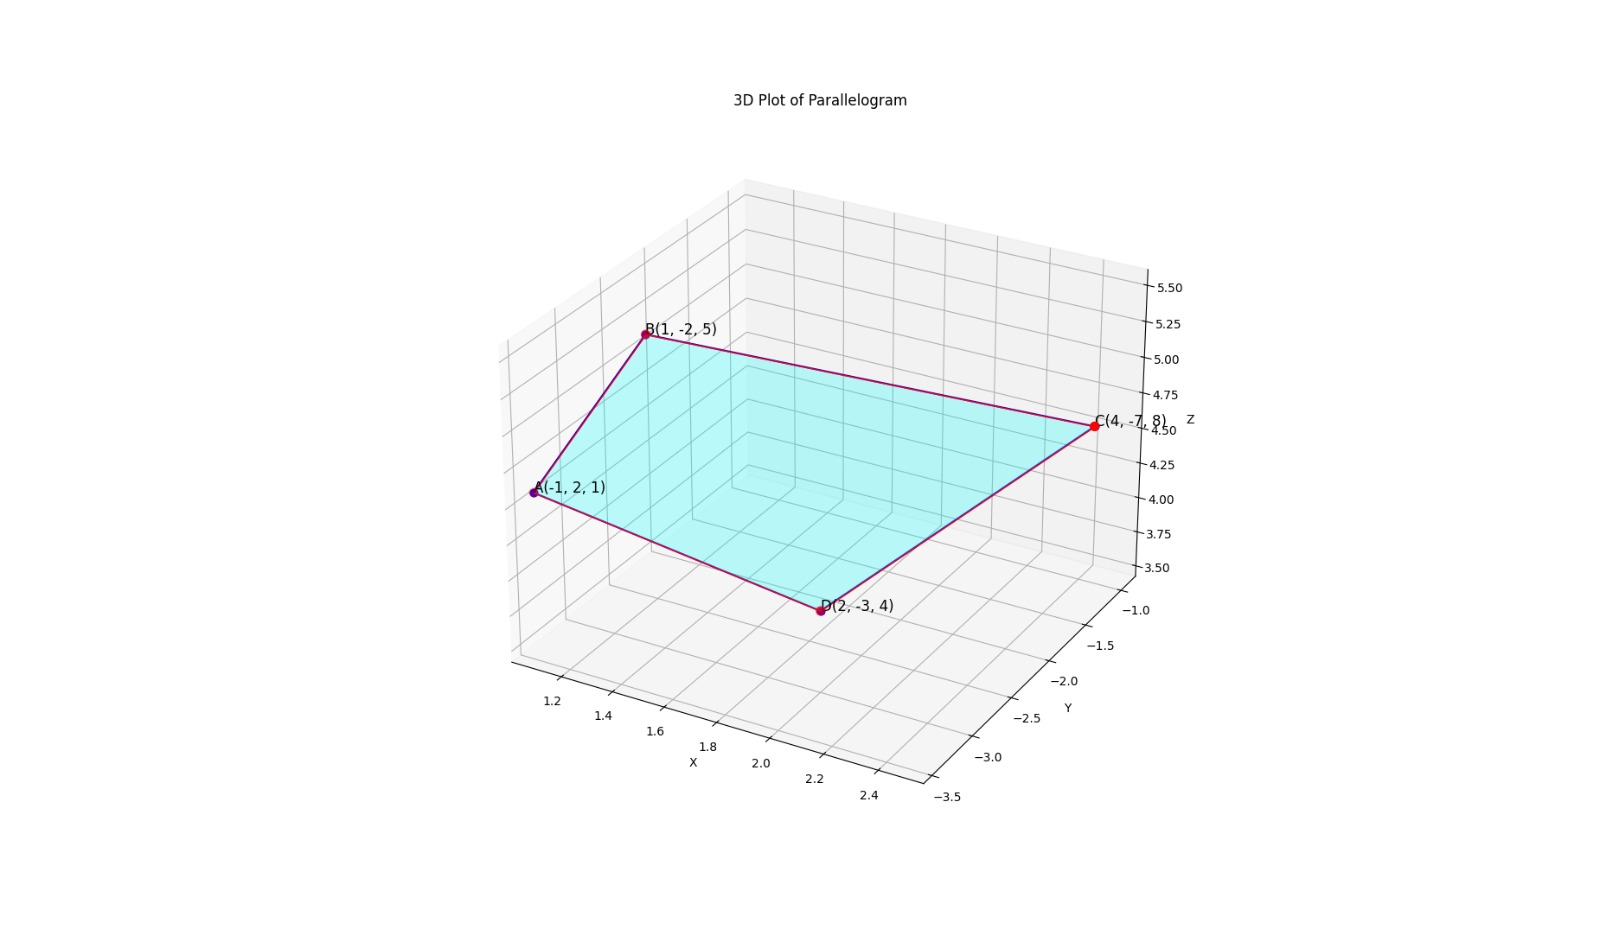
\includegraphics[width=1.1\linewidth]{IMG.jpg}
   \caption{Stem Plot of y\brak{n}}
     \label{stemplot}
\end{figure}


\end{document}  
